\documentclass{article}
\usepackage[utf8]{inputenc}
\usepackage[russian]{babel}
\usepackage{graphicx}
\usepackage{wrapfig}
\usepackage{float}

\graphicspath{ {./data/images} }
\author{Александр Романов Б01-107}
\date{}
\title{3.6.1 Спектральный анализ электрических сигналов.}

\begin{document}
\maketitle
\section{Введение}
\subsection{Цель работы}
Изучить спектральный состав периодических электриче­
ских сигналов.
\subsection{В работе используются} 
Анализатор спектра, генератор прямоугольных импульсов и сигналов специальной формы,
осциллограф.

\subsection{Идеи}
\subsubsection{Разложение сложных сигналов в ряд Фурье}
Для математического представления сложных периодических сигналов часто используют их представление
в виде линейной комбинации синусов и косинусов (Разложение в ряд Фурье). Например, если функция 
некоторого сигнала $s$ имеет частоту повторения \(\Omega = \frac{2\pi}{T}\), то её математическое
представление может быть найдено в виде:

\[ s(t) = \frac{a_0}{2} + \sum_{n=1}^{\infty}\left(a_n \cos n\Omega t + b_n \sin n\Omega t\right) \]

С коэффициентами:

\[ a_n = \frac{2}{T} \int_{-T/2}^{T/2}s(t) \cos n \Omega t dt  \]
\[ b_n = \frac{2}{T} \int_{-T/2}^{T/2}s(t) \sin n \Omega t dt  \]

Каждую гармонику можно описать её амплитудой \( A_n = \sqrt{a_n^2 + b_n^2} \) и начальной фазой 
\( \phi_n = arctg(b_n / a_n) \)

\subsubsection{Периодическая последовательность прямоугольных импульсов}


\begin{figure}[H]
\centering
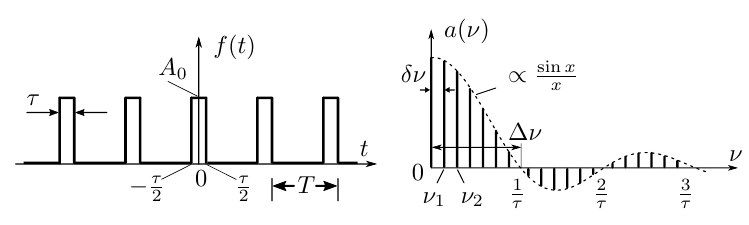
\includegraphics[width=\textwidth]{square_imp_example.png}
\caption{Периодическая последовательность прямоугольных импульсов и её спектр.} 
\label{sq_imp}
\end{figure}
Рассмотрим сигнал на рис \ref{sq_imp}.
Введем величину \( \Omega = \frac{2\pi}{T} \), где $T$ - частота повторения импульсов. $\tau$ - 
длительность импульса. Сигнал чётный, поэтому в ряде ненулевыми будут только коэффициенты при косинусах:

\[ a_n = \frac{2}{T} \int_{-\tau/2}^{\tau/2} A_o \cos \left(n\Omega t\right) dt  = 
2A_o \frac{\tau}{T}\frac{\sin \left(n\Omega\tau/2\right)}{n\Omega\tau/2} \sim 2A_o\frac{\tau}{T}\]

где $A_0$ - амплитуда сигнала.
Огибающая зануляется при \( n = \frac{2\pi}{\tau\Omega} \). Пусть $T$ кратно $\tau$. Введём величину $\Delta\nu$ - 
расстояние до первого нуля огибающей(характерная ширина спектра). И $\delta\nu$ - расстояние между
двумя соседними спектральными пиками. Имеют место "соотношения неопределённости":

\[ \Delta\nu\tau \simeq 1 \]
\[ \delta\nu T \simeq 1 \]

\subsubsection{Периодическая последовательность цугов гармонических колебаний}

\begin{figure}[H]
    \centering
    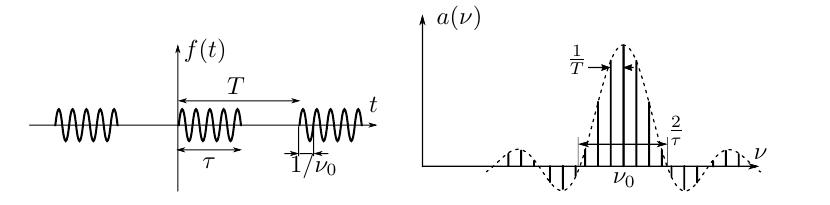
\includegraphics[width=\textwidth]{cug_imp_example.png}
    \caption{Периодическая последовательность прямоугольных импульсов и её спектр.} 
    \label{cug_imp_example}
\end{figure}

Рассмотрим сигнал на рис \ref{cug_imp_example}. Это - цуги колебания \( A_0 \sin \left(\nu_0t\right) \)
Снова пусть $T$ кратно $\tau$. Тогда Спектры последовательности идентичны прямоугольным импульсам, но
сдвинуты на $\nu_0$. Соотношения неопределённости остаются прежними:

\[ \Delta\nu\tau \simeq 1 \]
\[ \delta\nu T \simeq 1 \]

\subsubsection{Амплитудно-модулированные колебания}
\begin{figure}[H]
    \centering
    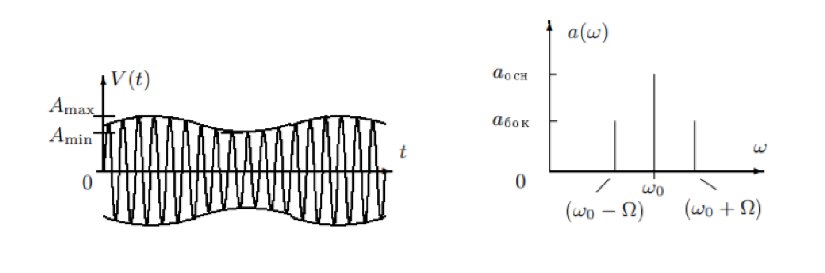
\includegraphics[width=\textwidth]{AM_signal_example.png}
    \caption{Амплитудно-модулированный сигнал и его спектр.} 
    \label{AM_sig_example}
\end{figure}

Рассмотрим (Рис. \ref{AM_sig_example}) гармонические колебания высокой частоты $\omega_0$, амплитуда которых
медленно меняется по гармоническому закону с частотой $\Omega \ll \omega$.

\[ s(t) = A_0\left[1 + m \cos \Omega t\right] \cos \omega_0 t \]

Коэффициент $m$ называется \emph{глубиной модуляции}. При \( m < 1 \) амплитуда меняется от минимальной 
\( A_{min} = A_0(1 - m) \) до максимальной \( A_{max} = A_0(1 + m) \). Глубина модуляции может быть представленна
в виде

\[ m = \frac{A_{max} - A{min}}{A_{max} + A_{min}}. \]

Отсюда можно легко переписать уравнение сигнала как:

\[ s(t) = A_0 \cos \omega_0t + \frac{A_0m}{2} \cos \left(\omega_0 + \Omega\right)t  + \frac{A_0m}{2} 
\cos \left(\omega_0 + \Omega\right)t.\]




\section{Работа}



\section{Выводы}
\end{document}